\documentclass[11pt,letterpaper]{article}
\usepackage{lltpaperstyle}
\usepackage{tikz}
\usepackage{calc}

\begin{document}

\section{Bullet Analysis and Measurements}

This document analyzes the current bullet implementation to understand exact measurements and appearance.

\subsection{Current Bullet Implementation}

\subsubsection{Standard Itemize (Gray Bullets)}

\begin{itemize}
\item Standard bullet with \texttt{bulletgray} at 20\% (0.20 gray = 80\% black)
\item The bullet symbol uses \texttt{\textbackslash textbullet} from TeX Gyre Pagella
\item Hanging indent: 1.8em, Label separation: 0.7em
\end{itemize}

\subsubsection{Bullet Symbol Comparison}

Let's compare different bullet implementations:

\begin{itemize}
\item[\textbullet] Pure black bullet (\texttt{\textbackslash textbullet})
\item[\textcolor{bulletgray}{\textbullet}] Current gray bullet at 20\% gray (80\% black)
\item[\textcolor{gray}[gray]{0.30}{\textbullet}] Lighter option at 30\% gray (70\% black)
\item[\textcolor{gray}[gray]{0.35}{\textbullet}] Even lighter at 35\% gray (65\% black)
\item[\textcolor{gray}[gray]{0.40}{\textbullet}] Subtle option at 40\% gray (60\% black)
\item[\textcolor{gray}[gray]{0.45}{\textbullet}] Original subtlegray at 45\% gray (55\% black)
\end{itemize}

\subsubsection{Alternative Bullet Symbols}

Comparing different bullet characters:

\begin{itemize}
\item[\textbullet] Standard \texttt{\textbackslash textbullet} (current)
\item[\textperiodcentered] Period centered \texttt{\textbackslash textperiodcentered}
\item[\scalebox{0.8}{\textbullet}] Scaled bullet at 80\%
\item[\scalebox{0.7}{\textbullet}] Scaled bullet at 70\%
\item[\raisebox{0.2ex}{\scalebox{0.6}{\textbullet}}] Scaled 60\% and raised
\item[$\bullet$] Math mode bullet
\item[$\cdot$] Math mode cdot
\item[\textopenbullet] Open bullet (if available)
\end{itemize}

\subsubsection{Measurement Analysis}

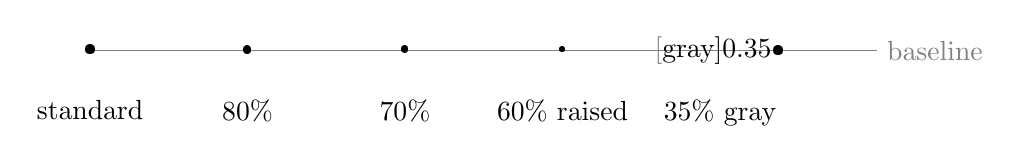
\begin{tikzpicture}[baseline]
  % Draw baseline
  \draw[gray,thin] (0,0) -- (10,0) node[right] {baseline};
  
  % Show bullet position
  \node at (0,0) {\textbullet};
  \node[below] at (0,-0.5) {standard};
  
  % Show scaled versions
  \node at (2,0) {\scalebox{0.8}{\textbullet}};
  \node[below] at (2,-0.5) {80\%};
  
  \node at (4,0) {\scalebox{0.7}{\textbullet}};
  \node[below] at (4,-0.5) {70\%};
  
  \node at (6,0) {\raisebox{0.15ex}{\scalebox{0.6}{\textbullet}}};
  \node[below] at (6,-0.5) {60\% raised};
  
  % Show color variations
  \node at (8,0) {\textcolor{gray}[gray]{0.35}{\textbullet}};
  \node[below] at (8,-0.5) {35\% gray};
\end{tikzpicture}

\subsection{Spacing Measurements}

Current spacing configuration:
\begin{description}
\item[Hanging indent] 1.8em = \the\listhangindent
\item[Label separation] 0.7em = \the\listlabelsep  
\item[Item separation] 3.3pt = \the\listquarterbaseline
\item[Top/bottom space] 6.6pt = \the\listhalfbaseline
\end{description}

\subsection{Optical Adjustments for Pagella}

TeX Gyre Pagella (Palatino-based) characteristics affecting bullets:
\begin{itemize}
\item Larger x-height than many fonts
\item Wider character proportions
\item Stronger stroke contrast
\item The standard \texttt{\textbackslash textbullet} appears heavier in Pagella
\end{itemize}

\subsection{Recommended Refinements}

Based on this analysis, potential improvements include:
\begin{enumerate}
\item Lighter gray: Move from 20\% to 30-35\% gray for subtler bullets
\item Smaller bullet: Scale to 70-80\% of standard size
\item Alternative symbol: Consider \texttt{\textbackslash textperiodcentered} raised slightly
\item Microtype tracking: Add slight negative tracking to bullet symbol
\end{enumerate}

\end{document}